\documentclass[10pt,pdf,hyperref={unicode}]{beamer}

\mode<presentation>
{
\usetheme{boxes}
\beamertemplatenavigationsymbolsempty

\setbeamertemplate{footline}[page number]
\setbeamersize{text margin left=1em, text margin right=0.5em}
}

\usepackage{algorithm}
\usepackage{algorithmicx}
\usepackage{algpseudocode}

\usepackage[utf8]{inputenc}
\usepackage[english, russian]{babel}
\usepackage[normalem]{ulem}
\usepackage{bm}
\usepackage{multirow}
\usepackage{ragged2e}
\usepackage{indentfirst}
\usepackage{multicol}
\usepackage{subfig}
\usepackage{amsmath,amssymb}
\usepackage{dsfont}
\usepackage{enumerate}
\usepackage{mathtools}
\usepackage{comment}
\usepackage{tabularx, tabulary, multicol}
\usepackage[all]{xy}

\newcommand{\bz}{\mathbf{z}}
\newcommand{\bx}{\mathbf{x}}
\newcommand{\by}{\mathbf{y}}
\newcommand{\bv}{\mathbf{v}}
\newcommand{\bw}{\mathbf{w}}
\newcommand{\ba}{\mathbf{a}}
\newcommand{\bb}{\mathbf{b}}
\newcommand{\bff}{\mathbf{f}}
\newcommand{\bh}{\mathbf{h}}
\newcommand{\bl}{\mathbf{l}}
\newcommand{\bp}{\mathbf{p}}
\newcommand{\bq}{\mathbf{q}}
\newcommand{\bs}{\mathbf{s}}
\newcommand{\bt}{\mathbf{t}}
\newcommand{\bu}{\mathbf{u}}
\newcommand{\bT}{\mathbf{T}}
\newcommand{\bX}{\mathbf{X}}
\newcommand{\bZ}{\mathbf{Z}}
\newcommand{\bS}{\mathbf{S}}
\newcommand{\bH}{\mathbf{H}}
\newcommand{\bW}{\mathbf{W}}
\newcommand{\bY}{\mathbf{Y}}
\newcommand{\bU}{\mathbf{U}}
\newcommand{\bQ}{\mathbf{Q}}
\newcommand{\bP}{\mathbf{P}}
\newcommand{\bA}{\mathbf{A}}
\newcommand{\bB}{\mathbf{B}}
\newcommand{\bC}{\mathbf{C}}
\newcommand{\bE}{\mathbf{E}}
\newcommand{\bF}{\mathbf{F}}
\newcommand{\bsigma}{\boldsymbol{\sigma}}
\newcommand{\bSigma}{\boldsymbol{\Sigma}}
\newcommand{\bomega}{\boldsymbol{\omega}}
\newcommand{\btheta}{\boldsymbol{\theta}}
\newcommand{\bgamma}{\boldsymbol{\gamma}}
\newcommand{\bdelta}{\boldsymbol{\delta}}
\newcommand{\bPsi}{\boldsymbol{\Psi}}
\newcommand{\bpsi}{\boldsymbol{\psi}}
\newcommand{\bxi}{\boldsymbol{\xi}}
\newcommand{\bmu}{\boldsymbol{\mu}}
\newcommand{\bchi}{\boldsymbol{\chi}}
\newcommand{\bzeta}{\boldsymbol{\zeta}}
\newcommand{\blambda}{\boldsymbol{\lambda}}
\newcommand{\beps}{\boldsymbol{\varepsilon}}
\newcommand{\bZeta}{\boldsymbol{Z}}
% mathcal
\newcommand{\cX}{\mathcal{X}}
\newcommand{\cY}{\mathcal{Y}}
\newcommand{\cW}{\mathcal{W}}

\newcommand{\dH}{\mathds{H}}
\newcommand{\dR}{\mathds{R}}
% transpose
\newcommand{\T}{^{\mathsf{T}}}

% command to strike out text
\newcommand{\stkout}[1]{\ifmmode\text{\sout{\ensuremath{#1}}}\else\sout{#1}\fi}

% limited alertblock
\newenvironment<>{varblock}[2][.9\textwidth]{%
	\setlength{\textwidth}{#1}
	\begin{actionenv}#3%
		\def\insertblocktitle{#2}%
		\par%
		\usebeamertemplate{block begin}}
	{\par%
		\usebeamertemplate{block end}%
	\end{actionenv}}

\renewcommand{\epsilon}{\ensuremath{\varepsilon}}
\renewcommand{\phi}{\ensuremath{\varphi}}
\renewcommand{\kappa}{\ensuremath{\varkappa}}
\renewcommand{\le}{\ensuremath{\leqslant}}
\renewcommand{\leq}{\ensuremath{\leqslant}}
\renewcommand{\ge}{\ensuremath{\geqslant}}
\renewcommand{\geq}{\ensuremath{\geqslant}}
\renewcommand{\emptyset}{\varnothing}

\usepackage{tikz}
\usetikzlibrary{positioning,arrows.meta,calc}
%\tikzstyle{naeme} = [parameters]
\definecolor{name}{rgb}{0.5,0.5,0.5}

\tikzset{
	myblock/.style = {draw, rounded corners, fill=blue!8, inner sep=4pt},
	myarrow/.style = {->, very thick, >=Stealth}
}

\usepackage{caption}
\captionsetup{skip=0pt,belowskip=0pt}

\newtheorem{rustheorem}{Теорема Владимирова}
\newtheorem{russtatement}{Утверждение}
\newtheorem{rusdefinition}{Определение}

% colors
\definecolor{darkgreen}{rgb}{0.0, 0.2, 0.13}
\definecolor{darkcyan}{rgb}{0.0, 0.55, 0.55}

\AtBeginEnvironment{figure}{\setcounter{subfigure}{0}}

\captionsetup[subfloat]{labelformat=empty}
\addto\captionsrussian{\renewcommand{\figurename}{}}
\graphicspath{{../figures/}}

%----------------------------------------------------------------------------------------------------------

\title[Заголовок]{Причинно-ориентированное снижение размерности для анализа данных нейроинтерфейсов}
\author{Владимиров Э.А.}

\institute[]{Московский физико-технический институт}
\date{\footnotesize
	\par\smallskip\emph{Научный руководитель:} д.~ф.-м.~н. В.\,В.~Стрижов
	\par\bigskip\small 2025}

%---------------------------------------------------------------------------------------------------------
\begin{document}

\begin{frame}
\titlepage
\end{frame}

%----------------------------------------------------------------------------------------------------------
\begin{frame}{Причинно-следственный анализ в данных высокой размерности}
	\begin{alertblock}{Проблема}
	    \begin{itemize}
			\item[-] Нелинейные, лагированные во времени зависимости не выявляются
			корреляцией и линейной регрессией.%
			\item[-] Высокая размерность данных усиливает мультиколлинеарность и усложняет поиск причинно-следственной сявзи
		\end{itemize}
	\end{alertblock}
	
	\begin{alertblock}{Цель исследования}
		Найти компактное и интерпретируемое скрытое пространство,
		в котором обнаруживается причинное воздействие $\bX \rightarrow \bY$.
	\end{alertblock}

	  \begin{alertblock}{Предлагаемая модель \textbf{CaSCA}}
	  	Предлагается подход CaSCA -- Канонический анализ каузальных подпространств.
	  	
	  	CaSCA проецирует данные на два взаимно ортогональных подпространства: \textbf{каузальное}, где лагированное представление $\bX$ 
	  	максимально предсказывает $\bY$, и \textbf{реконструктивное}, которое объясняет остаточную дисперсию сигналов.
		
	\end{alertblock}
\end{frame}

%---------------------------------------------------------------------------------------------------------
\begin{frame}{Основная идея метода CaSCA}

	\textbf{Ключевая мысль:} \\
	\emph{CaSCA строит общее латентное пространство, где на первом этапе извлекаются низкоразмерные причинные компоненты, а на втором — восстанавливается остальная вариативность данных.}
\end{frame}

%--------------------------------------------------------------------------------------------------------

\begin{frame}{Постановка задачи каузального снижения размерности}
	Даны два синхронных многомерных временных ряда \(\bX_t\in\mathbb{R}^{n_x},\;
			\bY_t\in\mathbb{R}^{n_y},\quad t=1,\dots,T\).
	
	\vspace{0.3em}
	Общий энкодер каждой строки
	\[
	\varphi_{\text{enc}}\!:\mathbb R^{n_x}\!\times\!\mathbb R^{n_y}\!\to\!\mathbb R^{m},
	\quad
	\psi_{\text{enc}}\!:\mathbb R^{n_x}\!\times\!\mathbb R^{n_y}\!\to\!\mathbb R^{m}
	\]
	создаёт скрытые представления
	\[
	\mathbf P_t = \varphi_{\text{enc}}(\mathbf X_t,\mathbf Y_t),\qquad
	\mathbf Q_t = \psi_{\text{enc}}(\mathbf X_t,\mathbf Y_t).
	\]
	
	\vspace{0.3em}
	\textbf{Разбиение скрытого пространства.}\;
	$m = d_{c}+d_{r}$,\;
	\(
	\mathbf P_t = \bigl[\mathbf P_t^{c} \;\vline\; \mathbf P_t^{r}\bigr],\;
	\mathbf Q_t = \bigl[\mathbf Q_t^{c} \;\vline\; \mathbf Q_t^{r}\bigr],
	\;
	\mathbf P_t^{c},\mathbf Q_t^{c}\in\mathbb R^{d_c},
	\;
	d_c\ll d_r\ll\min(n_x,n_y).
	\)
	
	\vspace{0.3em}
	\textbf{Декодеры и реконструкция.}\;
	\[
	\widehat{\mathbf X}_t = \varphi_{\text{dec}}\!\bigl(\mathbf P_t\bigr),\qquad
	\widehat{\mathbf Y}_t = \psi_{\text{dec}}\!\bigl(\mathbf Q_t\bigr).
	\]
	
\end{frame}


\begin{frame}{Постановка задачи каузального снижения размерности}
	Необходимо построить \emph{низкоразмерное} и \emph{причинно-информативное} латентное пространство, в котором
	\begin{itemize}
			\item[-] причинные компоненты (\(\bP_t^{\mathrm c},\bQ_t^{\mathrm c}\))  
			максимально объясняют влияние \(\bX_{t-\tau}\!\to\bY_t\);
			\item[-] реконструктивные компоненты (\(\bP_t^{\mathrm r},\bQ_t^{\mathrm r}\))  
			сохраняют оставшуюся дисперсию сигналов;
		\end{itemize}
	
	\textbf{Задача моделирования}
	
	Найти преобразования $\varphi_{\text{enc}}, \psi_{\text{enc}}, \varphi_{\text{dec}}, \psi_{\text{dec}}$,  
	минимизируя
	\[
	\mathcal{L}
	= \lambda_{\text{rec}}
	\bigl(
	\lVert\bX_t\!-\widehat{\bX}_t\rVert_F
	+ \lVert\bY_t\!-\widehat{\bY}_t\rVert_F
	\bigr)
	+ \lambda_{\text{c}}\,
	\mathcal{L}_{\text{c}}
	\!\bigl(\bP_{t-\tau}^{\mathrm c},\bQ_t^{\mathrm c}\bigr),
	\]
	\begin{itemize}
		\item[-] $\mathcal{L}_{\text{c}}$ — критерий причинно-следственной связи (корреляция/CCM/MI).
	\end{itemize}
	
	\textbf{Предположения.}
	\begin{itemize}
		\item[-] Аттрактор допускает задержанное вложение при умеренном шуме.
		\item[-] Вся значимая причинная информация содержится в $d_c$-мерном подпространстве.
		\item[-] Задержка $\tau$ заранее известна.
	\end{itemize}
\end{frame}

\begin{frame}{Критерии качества модели снижения размерности}
	\small
	
	\textbf{1. Устранение мультиколлинеарности}
		\begin{itemize}
			\item[] Максимальный Variance Inflation Factor (VIF) \; $\displaystyle \max_j \frac{1}{1-R_j^{2}}$
			\item[] Condition Number \; $\max(\kappa(\bP_t\T \bP_t), \kappa(\bQ_t\T \bQ_t)) = 
			\tfrac{\sigma_{\max}}{\sigma_{\min}}$
		\end{itemize}
	Чем меньше — тем более устойчивы линейные модели в скрытом пространстве
	
	\vspace{0.4em}
	
	\textbf{2. Точность реконструкции сигналов}
		\begin{itemize}
			\item[] $\displaystyle 
			\text{RMSE}_X = \sqrt{\tfrac1T \sum_t \lVert 
				\widehat{\bX}_t - \bX_t \rVert^2}\,$  (аналогично для $\bY$)
			\item[] Explained Variance Ratio — доля дисперсии, восстановленная  декодером
		\end{itemize}
	
	\vspace{0.4em}
	
	\textbf{3. Прогностическая полезность причинных эмбеддингов}
		\begin{enumerate}
			\item[(i)] модель $Y_{t}$ по собственным лагам $\bY_{t-\tau}$
			\item[(ii)] модель $Y_{t}$ по $\bY_{t}$ и исходным $\bX_{t}$
			\item[(iii)] модель $Y_{t}$ по $\bY_{t}$ и причинным эмбеддингам $\bP_{t}^{\mathrm c}$
		\end{enumerate}
		\[
		\Delta\!\text{Score} \;=\;
		\text{Perf}(\text{модель (iii)}) -
		\max\bigl\{\text{Perf}(\text{(i)}),\text{Perf}(\text{(ii)})\bigr\}
		\]
		\begin{itemize}
			\item $\text{Perf}$ — снижение RMSE / рост $R^2$ или F1 (для классификации)
		\end{itemize}
	
\end{frame}


%------------------------------------------------------------
\begin{frame}[fragile]{Алгоритм {\normalfont CaSCA}}
	\small
	\vspace*{-0.4em}
	\begin{algorithm}[H]   % пакет algorithm уже подключён в преамбуле
		\caption*{\textbf{CaSCA: причинно-ориентированное снижение размерности}}
		\begin{algorithmic}[1]
			\Require Временные ряды $\bX_t\in\dR^{T\times n_x},\;\bY_t\in\dR^{T\times n_y}$,
			лаги $\mathcal T$, размерности $d_c, d_{\text{hid}}$ 
			\Ensure  Кaузальные проекции $\bP_t^{\mathrm c},\bQ_t^{\mathrm c}$,  
			реконструктивные проекции $\bP_t^{\mathrm r},\bQ_t^{\mathrm r}$
			
			\Statex\textbf{Шаг 1.} \textit{Автовыбор лага}
			\For{$\tau\in\mathcal T$}
			\State $\rho(\tau)\gets\text{corr}\!\bigl(\text{CCA}_1(\bX_{t-\tau},\bY_t)\bigr)$
			\EndFor
			\State $\tau^\star\gets\arg\max_{\tau}\rho(\tau)$
			
			\Statex\textbf{Шаг 2.} \textit{Канонический блок (каузальный)}
			\State $\bigl[\bW_x^{\mathrm c},\bW_y^{\mathrm c}\bigr]\gets
			\text{CCA}\!\bigl(\bX_{t-\tau^\star},\bY_t,\;d_c\bigr)$
			\State $\bP_t^{\mathrm c}\!\gets\bX_t\bW_x^{\mathrm c}$, 
			$\bQ_t^{\mathrm c}\!\gets\bY_t\bW_y^{\mathrm c}$
			
			\Statex\textbf{Шаг 3.} \textit{Дефляция остатка}
			\State $\bX_{\text{res}}\gets\bX_t - \bP_t^{\mathrm c}{\bW_x^{\mathrm c}}^{\!\top}$, $\bY_{\text{res}}\gets\bY_t - \bQ_t^{\mathrm c}{\bW_y^{\mathrm c}}^{\!\top}$
			
			\Statex\textbf{Шаг 4.} \textit{PCA-блок (реконструктивный)}
			\State $\bW_x^{\mathrm r}\gets\text{PCA}\bigl(\bX_{\text{res}},\,d_r\bigr)$, 
			$\bW_y^{\mathrm r}\gets\text{PCA}\bigl(\bY_{\text{res}},\,d_r\bigr)$
			\State $\bP_t^{\mathrm r}\!\gets\bX_{\text{res}}\bW_x^{\mathrm r}$, \;
			$\bQ_t^{\mathrm r}\!\gets\bY_{\text{res}}\bW_y^{\mathrm r}$
		\end{algorithmic}
	\end{algorithm}
	
%\textbf{Шаг 5.} \textit{Реконструкция (опционально)}
%$\widehat{\bX}_t=\bar\bX+\bP_t^{\mathrm c}{\bW_x^{\mathrm c}}^{\!\top}
%+\bP_t^{\mathrm r}{\bW_x^{\mathrm r}}^{\!\top}$
%$\widehat{\bY}_t=\bar\bY+\bQ_t^{\mathrm c}{\bW_y^{\mathrm c}}^{\!\top}
%+\bQ_t^{\mathrm r}{\bW_y^{\mathrm r}}^{\!\top}$
%	\vspace{-0.8em}
%	\begin{itemize}\setlength\itemsep{2pt}
%		\item \textbf{Ключевая идея:} сначала извлекаем наиболее "прогностические"
%		направления (каузальные), затем в ортогональном остатке — наиболее 
%		информативные реконструктивные оси. 
%		\item Метод легко расширяется: заменить линейные $\varphi_{\text{enc}}/\psi_{\text{enc}}$ 
%		на нейросети, добавить CCM-регуляризатор и т.д.
%	\end{itemize}
\end{frame}
%------------------------------------------------------------

\begin{frame}{Теоретические свойства модели CaSCA}
	
	\begin{rustheorem}[2025, ортогональность и блочная дисперсия]
		Пусть после центрирования данные приведены к единичной ковариации  
		$\Sigma_{XX}=I_p,\;\Sigma_{YY}=I_q$. 
		Тогда проекции $\bP_t^c, \bP_t^r$ и ортогональные веса $\bW_x^c, \bW_x^r$ модели обладают следующими свойствами:
		
		\begin{enumerate}
			\item \textbf{Ортогональность весов: }\;
			$W_x^{{\mathrm c}\top}W_x^{\mathrm r}=0_{d_c\times d_r}$  
			и аналогично для $Y$-блока.  
			\item \textbf{Разложение ковариации: }\;
			$I_p = \bW_x^{\mathrm c}\Sigma_{pp}^{\mathrm cc}\bW_x^{{\mathrm c}\top}
			+ \bW_x^{\mathrm r}\Sigma_{pp}^{\mathrm rr}\bW_x^{{\mathrm r}\top}$  
			(кросс-блочные элементы обнуляются).  
			\item \textbf{Независимость латентных координат: }\;
			$\bP_t^{\mathrm c\top}\bP_t^{\mathrm r}=0_{d_c\times d_r}$,  
			т.е. причинные и реконструктивные факторы некоррелированы.
		\end{enumerate}
	\end{rustheorem}
	
	\vspace{-0.6em}
	\textbf{Интерпретация.}
	\begin{itemize}
		\item[] Причинные оси $\bW^{\mathrm c}$ изолируют подпространство, достаточное для прогноза $\bY_t$ по $\bX_{t-\tau}$.
		\item[] Реконструктивные оси $W^{\mathrm r}$ содержат остаточную дисперсию, не мешая оценке причинных связей.
		\item[] Блочное разложение дисперсии упрощает прикладные модели:  
		$\bP_t^{\mathrm c}$ используется в регрессии/классификации,  
		$\bP_t^{\mathrm r}$ — в реконструкции и фильтрации шума.
	\end{itemize}
\end{frame}


%------------------------------------------------------------
\begin{frame}{Переход в траекторное пространство}
	Вместо исходных наблюдений $\bX_t,\bY_t$ строим их отложенные векторы и применяем \textbf{CaSCA} уже к этим псевдонаблюдениям.
	Это раскрывает внутреннюю динамику системы и улучшает выявление причинных связей.
	
%	\vspace{0.8ex}
	\begin{algorithmic}[1]
		\Require{временные ряды $\{\bX_t\}_{t=1}^T,\{\bY_t\}_{t=1}^T$,  
			лаговое окно $E,\tau$}
		\Statex\textbf{Шаг 1.} \textit{Построение траекторий}
		\State $\displaystyle
		\bX^{(\mathrm{traj})}_t
		\!=\!
		\bigl[\bX_t,\bX_{t-\tau},\dots,\bX_{t-(E-1)\tau}\bigr]$
		\State Аналогично $\bY^{(\mathrm{traj})}_t$
		\Statex\textbf{Шаг 2.} \textit{Применение CaSCA}
		\State $(\bP^{\!\mathrm c},\bP^{\!\mathrm r},
		\bQ^{\!\mathrm c},\bQ^{\!\mathrm r})
		\leftarrow\text{CaSCA}
		\bigl(\bX^{(\mathrm{traj})},\,\bY^{(\mathrm{traj})}\bigr)$
		\Statex
		\Statex\textbf{Шаг 3.} \textit{Восстановление сигналов}
		\State $\widehat{\bX}_t =\,
		\overline{\bX}\;
		+\bP_t^{\!\mathrm c}\,W_x^{\mathrm c\T}
		+\bP_t^{\!\mathrm r}\,W_x^{\mathrm r\T}$
		\State аналогично $\widehat{\bY}_t$
	\end{algorithmic}
\end{frame}
%------------------------------------------------------------

\begin{frame}{Переход в траекторное пространство}

\begin{center}
	\begin{tikzpicture}[
		every node/.style={font=\footnotesize, align=center},
		>=Stealth,                    % <-- используем Stealth-стрелки
		node distance=8mm and 12mm    % базовый отступ между узлами
		]
		% Исходные ряды X_t, Y_t
		\node (X) {$\bX_t$};
		\node[right=of X] (Y) {$\bY_t$};
		
		% Блок построения лагового пространства
		\node[draw, below=of $(X)!0.5!(Y)$, minimum width=30mm] (lag) {Lag space};
		
		% Выходы (которые являются задержанными траекториями)
		\node[below left=of lag] (Xtraj) {$\bX_t^{\mathrm{traj}}$};
		\node[below right=of lag] (Ytraj) {$\bY_t^{\mathrm{traj}}$};
		
		% Блок CaSCA
		\node[draw, below=of lag, minimum width=40mm, yshift=-3mm] (casc) {CaSCA};
		
		% Латентные (скрытые) компоненты
		% В качестве примера выносим их на одну линию ниже CaSCA
		\node[below left=of casc, xshift=8mm, yshift=-2mm] (Pc) {$\bP_t^{\mathrm c}$};
		\node[below right=of casc, xshift=-8mm, yshift=-2mm] (Qc) {$\bQ_t^{\mathrm c}$};
		
		% Для наглядности (необязательно):
		\node[below=of Pc] (Pr) {$\bP_t^{\mathrm r}$};
		\node[below=of Qc] (Qr) {$\bQ_t^{\mathrm r}$};
		
		% Рисуем стрелки
		\draw[->] (X) -- (lag);
		\draw[->] (Y) -- (lag);
		\draw[->] (lag) -- (Xtraj);
		\draw[->] (lag) -- (Ytraj);
		
		\draw[->] (Xtraj) -- (casc);
		\draw[->] (Ytraj) -- (casc);
		
		\draw[->] (casc) -- (Pc);
		\draw[->] (casc) -- (Qc);
		\draw[->] (Pc) -- (Pr);
		\draw[->] (Qc) -- (Qr);
	\end{tikzpicture}
\end{center}

	\vspace{0.4ex}
	\textbf{Преимущество}: вложение Таккенса отображает исходные временные ряды в траекторное пространство, где нелинейные и запаздывающие взаимодействия становятся линейно отделимыми.
	В этом пространстве CaSCA извлекает ортогональные причинные координаты даже при больших лагах.
\end{frame}

\begin{frame}{Переход в Риманово пространство}
	\small
	\begin{columns}[T]
		%---------- LEFT  --------------------------------
	\begin{column}{0.55\textwidth}
		\begin{block}{Мотивация}
			\begin{itemize}\setlength{\itemsep}{3pt}
				\item EEG-сигналы многоканальны, шумны и содержат коррелированные компоненты.
				\item Ковариационные матрицы каналов естественно живут на многообразии SPD$(n)$.
				\item Проекция в касательное пространство = «локальная евклидизация»: работает линейная CaSCA.
			\end{itemize}
		\end{block}
		
		\begin{block}{Пошаговый алгоритм}
			\small
			\begin{enumerate}\setlength{\itemsep}{2pt}
				\item \textbf{XdawnCovariance.}\;  
				Из $N$ каналов формируем $n\! \ll\! N$ пространственных паттернов  
				$\,\bSigma_t\!\in\!\operatorname{SPD}(n)$ внутри окна $\Delta t$.
				\item \textbf{Log-Tangent.}\;
				$$\bC_t=\log\!\bigl(\bSigma_\star^{-1/2}\,\bSigma_t\,\bSigma_\star^{-1/2}\bigr)
				\;\in\;T_{\bSigma_\star}\operatorname{SPD}(n),$$
				где $\bSigma_\star$ — геометрическое среднее.
				\item \textbf{Сдвиг-матр. задержек.}\;
				Строим траекторию ${\bC}_{t,\tau}=[\bC_t,\,\bC_{t-\tau},\dots]$ и нормируем.
				\item \textbf{CaSCA.}\;  
				Применяем алгоритм из предыдущего слайда к парам 
				$(\bC^X_{t,\tau},\;\bC^Y_{t,\tau})$ $\Rightarrow$
				получаем причинные и реконструктивные эмбеддинги.
			\end{enumerate}
		\end{block}
	\end{column}
	
	%---------- RIGHT  -------------------------------
	\begin{column}{0.43\textwidth}
%			\begin{center}
%				\includegraphics[width=\linewidth]{figures/riem_traj.pdf}
%			\end{center}
		\begin{varblock}[0.9\linewidth]{Ключевая идея}
			Ковариации EEG являются точками на кривой SPD-многообразия;  
			перевод в касательное пространство делает их «плоскими»,  
			после чего CaSCA отделяет \textit{динамически-причинные} направления  
			от \textit{реконструктивного шума}.
		\end{varblock}
		
		\vspace{0.2em}
		\begin{varblock}{Итоговые преимущества}
			\begin{itemize}\setlength{\itemsep}{2pt}
				\item[] Устойчивость к масштабированию и к артефактам отдельных электродов.
				\item[] Геометрически корректная обработка SPD-данных.
				\item[] Улучшенная предсказательная точность $\uparrow$ (см. раздел экспериментов).
			\end{itemize}
		\end{varblock}
	\end{column}
	\end{columns}
\end{frame}
%
%\begin{frame}{Расширение CaSCA на глубокие сети}
%	\small
%	Заменяем линейную пару $\varphi_{\mathrm{enc}},\psi_{\mathrm{enc}}$ на двухголовый \textbf{Cross-Attention}  (CA) --  она одновременно учится находить канонические представления,  реализует задержки благодаря механизмам self-attention.
%	
%	\begin{varblock}{Модель \textit{Deep-CaSCA}}
%		\vspace{-0.2em}
%		\begin{enumerate}
%			\item[] \textbf{Кодеры}:  
%			$(P_t^{c},P_t^{r})=\Phi_{\theta}(\!\bX_{1:t}),\;
%			(Q_t^{c},Q_t^{r})=\Psi_{\theta}(\!\bY_{1:t})$ — трансформеры с CA-блоками.  
%			\item[] \textbf{Декодеры}:  
%			$\widehat{\bX}_t=\Phi^{-1}_{\theta}(P_t^{r}),\;
%			\widehat{\bY}_t=\Psi^{-1}_{\theta}(Q_t^{r})$.  
%			\item[] \textbf{Функция потерь}:  
%			\[
%			\mathcal L \;=\; \lambda_{\text{rec}}
%			\bigl[\!\| \bX-\widehat{\bX}\|_F + \| \bY-\widehat{\bY}\|_F \bigr]\;
%			+\;\lambda_{\text{c}}\,
%			\underbrace{ \bigl(1-\text{corr}(P^{c},Q^{c})\bigr) }_{\text{\scriptsize «CCM–loss»}}
%			\]
%			где \texttt{corr} вычисляется батчево.
%		\end{enumerate}
%	\end{varblock}
%\end{frame}
%
%
%\begin{frame}{Расширение CaSCA на глубокие сети}
%	\begin{rustheorem}[2024, Эквивалентность CA и CCA]
%		Пусть $\,\mathrm{CA}_k(\bX,\bY)$ — одноголовая cross-attention без нелинейностей c $k$ ключами.  
%		Если \,$\bX,\bY$ предварительно ортогонализованы, то  
%		выходные представления \,$U=\mathrm{CA}_k(\bX,\bY),\;V=\mathrm{CA}_k(\bY,\bX)$  
%		максимизируют выборочную корреляцию так же, как первые $k$ канонических пар CCA.
%	\end{rustheorem}

%	\vspace{0.5em}
%	Cross-attention обучается поворачивать скрытое пространство так, чтобы каждая голова совпадала с каноническим направлением; сам механизм self-attention неявно реализует сдвиги $\bX_{t-\tau}$ $\!\!\rightarrow$ $\bX_{t}$.
%\end{frame}
%%------------------------------------------------------------
%
%%--------------------------------------------------
%\begin{frame}{Регуляризатор Сугихары: вспоминаем метод}
%	\begin{varblock}{Сходящийся перекрестный анализ}
%			\textbf{Теневое вложение:}
%		\[
%		M_{X,t}
%		= 
%		\bigl(
%		X_t,\,
%		X_{t-\tau},\,
%		\dots,\,
%		X_{t-(E-1)\tau}
%		\bigr)
%		\;\in\;\mathbb{R}^E,
%		\]
%		где $E$ --- размерность вложения, $\tau$ --- временной лаг. 
%		%Аналогично задаётся $M_{Y,t} = \bigl(Y_t,\,Y_{t-\tau},\,\dots\bigr).$
%		
%		\vspace{1em}
%		\textbf{Реконструкция:}
%		\[
%		\widehat{Y}_t | M_{X, t}
%		=
%		\sum_{i=1}^{k}
%		w_i\,
%		Y_{n_i},
%		\]
%		здесь $n_i$ --- индексы ближайших соседей точки $M_{X,t}$ в пространстве $M_X$, а $w_i$ --- веса, зависящие от расстояния до $M_{X,t}$.
%		
%		\vspace{1em}
%		\textbf{Критерий причинности:}
%		\[
%		\rho_{X\to Y}
%		=
%		\mathrm{corr}\!\Bigl( Y_t, \widehat{Y}_t | M_{X, t} \Bigr).
%		\]
%		Если при увеличении размера ``библиотеки'' (множества рассматриваемых соседей) $\rho_{X \to Y}$ \emph{сходится монотонно}, считается, что $\mathbf{X}(t)$ влияет на $\mathbf{Y}(t)$.
%	\end{varblock}
%\end{frame}
%
%
%\begin{frame}{Регуляризатор Сугихары: статистические тесты сходимости}
%	Проверяем, что $\rho_{X\to Y}(L)$ \;«устойчиво растёт» при увеличении длины библиотеки $L$
%	\begin{itemize}
%		\item[] \textbf{Шаг 1.} Формируем последовательность оценок
%		\[
%		\rho_{X\to Y}(L_0),\;
%		\rho_{X\to Y}(L_1),\dots,
%		\rho_{X\to Y}(L_{\max}), \quad
%		L_0=E,\;L_{\max}=T .
%		\]
%		\item[] \textbf{Шаг 2.} \emph{Тест Кендалла $\tau$}  
%		— проверяем наличие значимого монотонного тренда  
%		$\rho_{X\to Y}(L_i)\nearrow$ при росте $L_i$.
%		
%		\[
%		H_0:\;\tau=0
%		\quad\Longrightarrow\quad
%		p_{\tau} < \alpha \;\;\text{(тренд есть)}
%		\]
%		
%		\item[] \textbf{Шаг 3.} \emph{Тест Фишера $\Delta\!Z$}  
%		— оцениваем, отличается ли
%		$\rho_{X\to Y}(L_{\max})$  
%		от  $\rho_{X\to Y}(L_{0})$ статистически значимо:
%		
%		\[
%		Z  \;=\; 
%		\frac{\operatorname{atanh}\rho(L_{\max})-\operatorname{atanh}\rho(L_{0})}
%		{\sqrt{\dfrac{1}{\,L_{\max}-3}+\dfrac{1}{\,L_{0}-3}}}, 
%		\qquad
%		p_{Z}<\alpha .
%		\]
%		
%		\item[] \textbf{Решение.}  Считаем кросс-мап подтверждённым, 
%		если одновременно \(p_{\tau}\) и \(p_{Z}\) меньше порога~\(\alpha\)
%		(обычно \(\alpha=0.05\)).
%	\end{itemize}
%\end{frame}
%
%
%\begin{frame}{Регуляризатор Сугихары: обучение с учётом динамики}
%%	\begin{varblock}{Зачем нужен регуляризатор ССМ?}
%%		\begin{itemize}
%%			\item[] Стандартная корреляция фиксирует лишь <<статические>> связи.  
%%			\item[] CCM проверяет \textbf{динамическую} причинность:  
%%			насколько траектория $M_{X,t}$ предсказывает $Y_t$ при
%%			увеличении размера библиотеки $L$.
%%			\item[] Включаем $-\rho_{X\to Y}(L_{\max})$ в целевую функцию,  
%%			чтобы модель \emph{конструктивно} усиливала истинную
%%			направленную зависимость.
%%		\end{itemize}
%%	\end{varblock}
%%
%%% ---------- RIGHT COLUMN : алгоритм ----------
%%	\begin{varblock}{Алгоритм обучения (псевдокод)}
%%		\begin{algorithmic}[1]
%%			\State \textbf{Input:} $\;X_t,\,Y_t;\,$ параметры сети
%%			\For{epoch = 1 \textbf{to} $E$}
%%			\State $P_t,\,Q_t \leftarrow$ encoders$(X_t,Y_t)$
%%			\State $\hat X_t,\hat Y_t \leftarrow$ decoders$(P_t,Q_t)$
%%			\State \textcolor{darkgreen}{$\rho \leftarrow$ CCM}\big($P_{t-\tau}^c,\,Q_t^c\big)$
%%			\State $\mathcal L_{\text{rec}} \gets
%%			||X-\hat X||_F + ||Y-\hat Y||_F$
%%			\State $\mathcal L \gets
%%			\lambda_{\text{rec}}\mathcal L_{\text{rec}}
%%			-\lambda_{\text{ccm}}\rho$
%%			\State back-propagate\;$(\mathcal L)$
%%			\EndFor
%%		\end{algorithmic}
%%	\end{varblock}
%	\small
%	\textbf{Цель CaSCA+CCM.}\;
%	Обучаемые параметры энкодеров/декодеров~$\,\varphi,\psi\,$
%	и весов~$A,B$ минимизируют
%	\[
%	\boxed{%
%		\mathcal L
%		=\;
%		\lambda_{\text{rec}}\,
%		\underbrace{%
%			\bigl(
%			\|{\bf X}_t-\widehat{\bf X}_t\|_F+
%			\|{\bf Y}_t-\widehat{\bf Y}_t\|_F
%			\bigr)
%		}_{\displaystyle \mathcal L_{\text{rec}}}
%		\;+\;
%		\lambda_{\rho}\,
%		\underbrace{%
%			\bigl(-\rho^{\text{CCM}}_{X\to Y}(A,B)\bigr)
%		}_{\text{causal\,score}}
%		\;+\;
%		\lambda_{\text{mono}}\,
%		P^{\text{mono}}
%		\;+\;
%		\lambda_{\text{gap}}\,
%		P^{\text{gap}} }
%	\]
%	
%	\vspace{0.6em}
%	\begin{enumerate}
%		\item \(\displaystyle \rho^{\text{CCM}}_{X\to Y}(A,B)
%		=\mathrm{corr}\!\Bigl(Y_t,\,
%		\widehat Y_t\,|\,M_{X,t}(A)\Bigr)\)
%		— «skill» перекрёстной реконструкции\\
%		(чем он выше, тем сильнее причинное влияние $\!X\!\to\!Y$).
%		
%		\item \(\displaystyle
%		P^{\text{mono}}
%		=\!
%		\sum_{i=2}^{|{\mathcal L}|}
%		\operatorname{softplus}\!\Bigl(
%		\rho(L_{i-1})-\rho(L_i)+\varepsilon
%		\Bigr)
%		\) — штраф за любое \emph{немонотонное} уменьшение
%		CCM-корреляции при увеличении объёма библиотеки
%		
%		\item \(\displaystyle
%		P^{\text{gap}}
%		=\operatorname{softplus}\!\Bigl(
%		\delta - \Delta z
%		\Bigr),\quad
%		\Delta z = z\!\bigl(\rho(L_{\max})\bigr) -
%		z\!\bigl(\rho(L_{\min})\bigr),
%		\;\;
%		z(p)=\tfrac12\ln\frac{1+p}{1-p}
%		\)\\[0.15em]
%		— штраф, если преобразованный
%		прирост корреляции между минимальной
%		и максимальной библиотеками
%		меньше заданного порога \(\delta\).
%	\end{enumerate}
%\end{frame}

%----------------------------------------------------------------------------------------------------------
\begin{frame}{Вычислительный эксперимент: описание данных}
	\begin{multicols}{2}
	
		\begin{varblock}[6cm]{Данные EEG-IMU}
			У 25 участников были записаны показания EEG, IMU, MRT во время игры в настольный теннис. С каждым участником было сыграно 4 сессии, длительность каждой из них составляет 7-10 минут.
		\end{varblock}
	
		\begin{figure}
			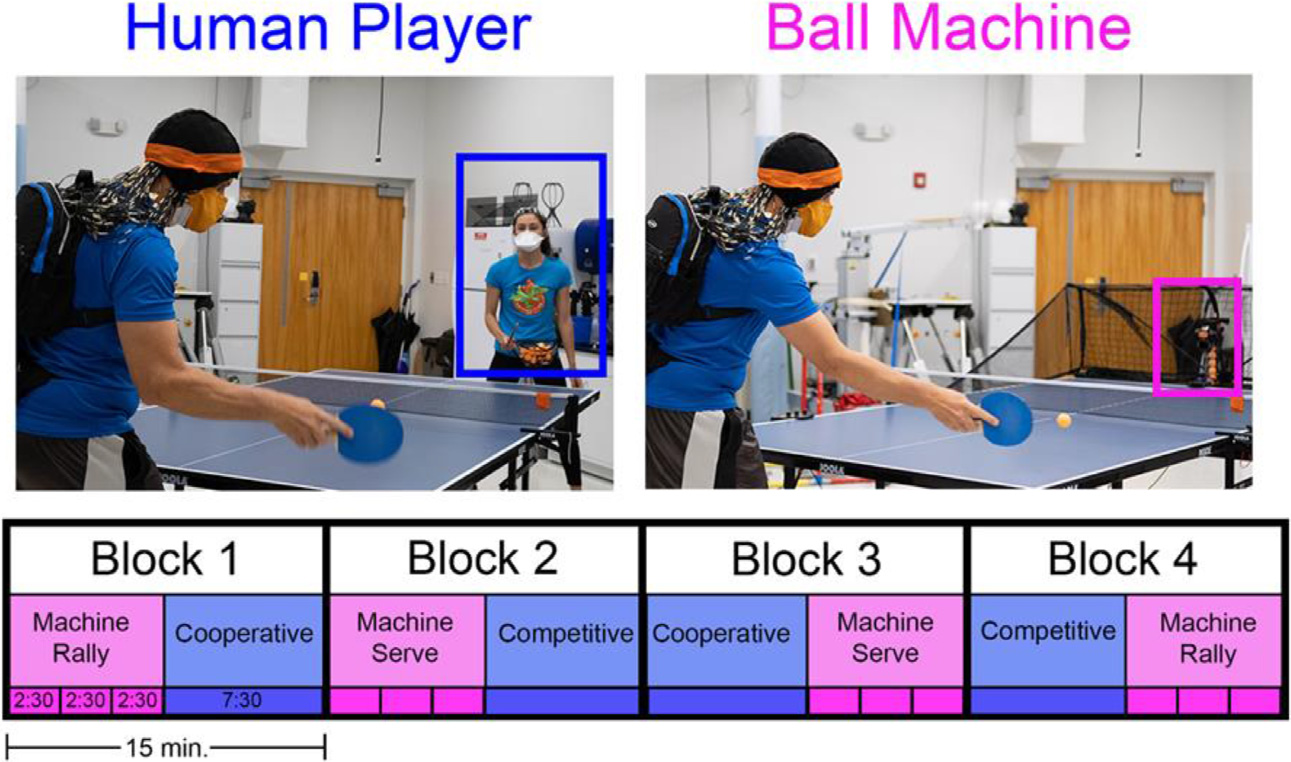
\includegraphics[width=\linewidth]{tennis-viz.png}
		\end{figure}
	
		\begin{varblock}[6cm]{Данные двух IMU устройств}
			Показания акселерометра и гироскопа со смартфона и планшета, записанные во время 10 минутной ходьбы.
		\end{varblock}
	
		\begin{figure}
			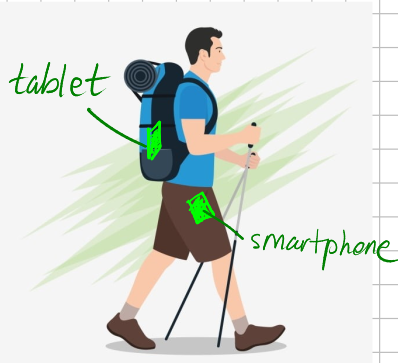
\includegraphics[width=\linewidth]{two-imu-devices.png}
		\end{figure}

	\end{multicols}
\end{frame}

\begin{frame}{Вычислительный эксперимент: сравнение CaSCA в исходном и траекторном пространствах}
	\begin{table}[]
		\begin{tabular}{lr|c|c|}
			\cline{3-4}
			& \multicolumn{1}{l|}{} & \multicolumn{1}{l|}{CaSCA} & \multicolumn{1}{l|}{CaSCA traj.} \\ \hline
			\multicolumn{1}{|l|}{kNN}           & Expl.var.ratio        & -3.4\%                     & -2.1\%                           \\ \hline
			\multicolumn{1}{|l|}{}              & RMSE                  & -0.11                      & -0.08                            \\ \hline
			\multicolumn{1}{|l|}{Linear}        & Expl.var.ratio        & -3.3\%                     & +0.3\%                           \\ \hline
			\multicolumn{1}{|l|}{}              & RMSE                  & -0.07                      & 0.01                             \\ \hline
			\multicolumn{1}{|l|}{Grad.Boosting} & Expl.var.ratio        & -0.7\%                     & -0.1\%                           \\ \hline
			\multicolumn{1}{|l|}{}              & RMSE                  & -0.026                     & -0.006                           \\ \hline
		\end{tabular}
	\end{table}
\end{frame}

\begin{frame}{Выносится на защиту}
	\begin{enumerate}
		\item
		Предложен причинный метод снижения размерности, 
		выделяющий отдельное латентное подпространство для
		причинных компонент и обеспечивающий точную реконструкцию сигналов.
		
		\item
		Доказано ортогональное разложение выборочной ковариации
		и строгая разделимость вариации на «причинный» и «реконструктивный» блоки в ортогональном пространстве состояний.
		
		\item
		Разработаны модификации метода в траекторном, римановом и
		глубоком обучающих пространствах, а такжee
		регуляризатор CCM, вводящий динамическое ограничение Сугихары
		через дифференцируемый штраф.
		
		\item
		Сформулирован комплекс метрических показателей
		(мультиколлинеарность, e, улучшение качества прогноза)  
		для объективного сравнения методов причинного анализа.
		e
		\item
		Проведены тесты на двух наборах данных
		(два IMU-датчика и EEG-IMU.
	\end{enumerate}
\end{frame}

\end{document} 
